\section{Parameter simulation}

\begin{itemize}
\item{Viable distances}
\item{Antenna Gains}
\item{Noises}
\item{Power receiver thresholds...}
\end{itemize}

As a first example the LOS maximum distance will be considered. This, as seen in section \ref{subsec:los_propagation}, depends on the altitude of the Ground Station and the altitude of the drone. Figure \ref{fig:altitude2distance} shows how the maximum distance in which there is still line-of-sight changes with the altitudes.

\begin{figure}[H]
	\centering
	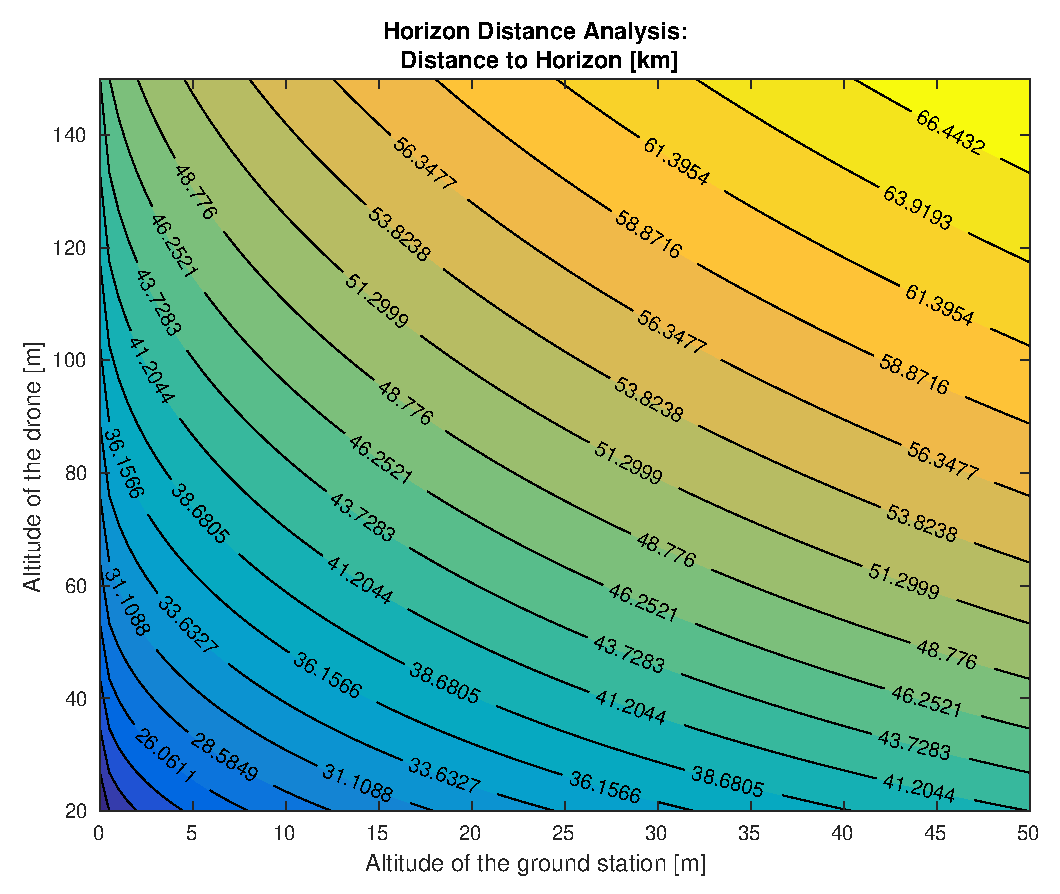
\includegraphics[scale=0.70]{figures/altitude2distance.eps}
	\caption{LOS distance parameter simulation}
   	\label{fig:altitude2distance}
\end{figure}

However this is not taking into consideration the relief of the Earth's surface, and therefore ignoring the obstacles that one could encounter in the real application. Thus, the next section will explain how a simulation was performed in order to take this into account.
